\documentclass[11pt]{article}

\usepackage{amsmath}
\usepackage{amssymb}
\usepackage{fancyhdr}
\usepackage{comment}
\usepackage{color}
\usepackage{graphicx}
\usepackage{tikz}
\usepackage[colorlinks=true,linkcolor=blue,urlcolor=blue]{hyperref}

\newcounter{marks}
\def\maxmarks#1{\extramark{#1}\addtocounter{marks}{#1}}
\def\extramark#1{
  \begin{flushright}
  [\emph{#1 points}]
  \end{flushright}
%  \quad\mbox{\LARGE\begin{tabular}{|c|c|}
%  \hline\rule{1cm}{0cm} & #1 \\ \hline \end{tabular}}
}
\def\dumptotal{%
\begin{flushright}
\begin{tabular}{|l|} \hline
\LARGE{\textbf{\rule{0pt}{16pt}Total:~\themarks}} \\ \hline
\end{tabular}
\end{flushright}}
\def\skiplines#1{\newline \forloop{#1}{{\rule{0pt}{20pt}} \\}}

\specialcomment{answer}{\color{blue}}{\color{black}}
\def\withanswers{\def\skiplines##1{\relax}\def\skippage{\relax}}
\def\withoutanswers{\excludecomment{answer}\def\skippage{\clearpage}}

\newif\ifprint
\printtrue

\oddsidemargin0cm
\topmargin-2cm     %I recommend adding these three lines to increase the 
\textwidth16.5cm   %amount of usable space on the page (and save trees)
\textheight23.5cm  

\newcommand{\mycoursenum}{10-601}
\newcommand{\myhwnum}{1}
\newcommand{\myname}{Dawei Wang}
\newcommand{\myandrew}{daweiwan@andrew.cmu.edu}
\newcommand{\myfirstta}{Abhinav Maurya}
\newcommand{\mysecondta}{Jingwei Shen}

\newcommand{\question}[2] {\vspace{.25in} \hrule\vspace{0.5em} \noindent{\bf #1: #2} \vspace{0.5em} \hrule \vspace{.10in}}
\renewcommand{\part}[1] {\vspace{.10in} {\bf (#1)}}

\setlength{\parindent}{0pt}
\setlength{\parskip}{5pt plus 1pt}
 
\pagestyle{fancyplain}
\lhead{\fancyplain{}{\textbf{HW\myhwnum}}}
\ifprint
\rhead{\fancyplain{}{Andrew ID: daweiwan}}
\else
\rhead{\fancyplain{}{\myname\\ \myandrew}}
\fi
\chead{\fancyplain{}{\mycoursenum}}

\withoutanswers

\begin{document}

\medskip

\thispagestyle{plain}
\begin{center}
{\Large \mycoursenum: Homework \myhwnum} \\
Due: 18 September 2014 11:59pm (Autolab) \\
TAs: \myfirstta, \mysecondta \\
\medskip
\ifprint
Name: Dawei Wang \\
Andrew ID: daweiwan \\
\else
Name: \myname \\
Andrew ID: \myandrew \\
\fi
\end{center}

Please answer to the point, and do not spend time/space giving irrelevant details. You should not require more space than is provided for each question. If you do, please think whether you can make your argument more pithy, an exercise that can often lead to more insight into the problem. Please state any additional assumptions you make while answering the questions. You need to submit a single PDF file on autolab. Please make sure you write legibly for grading.

You can work in groups. However, no written notes can be shared, or taken during group discussions. You may ask clarifying questions on Piazza. However, under no circumstances should you reveal any part of the answer publicly on Piazza or any other public website. The intention of this policy is to facilitate learning, not circumvent it. Any incidents of plagiarism will be handled in accordance with \href{http://www.cmu.edu/policies/documents/Academic%20Integrity.htm}{CMU's Policy on Academic Integrity}.


%%%%%%%%%%%%%%%%%%%%%%%%%%%%%%%%%%%%%%%%%%%
\question{$\star$}{Code of Conduct Declaration}

\begin{itemize}
	\item Did you receive any help whatsoever from anyone in solving this assignment? {\bf Yes}.
	\item If you answered \emph{yes}, give full details: {\it Alvin provided me with some insights on problem 5}. 
	\item Did you give any help whatsoever to anyone in solving this assignment? {\bf Yes}.
	\item If you answered \emph{yes}, give full details: {\it I helped Graeme with problem 1 and 3}.
\end{itemize}


%%%%%%%%%%%%%%%%%%%%%%%%%%%%%%%%%%%%%%%%%%%
\question{1}{The truth will set you free. (TA:- \myfirstta)}

State whether true (with a brief reason) or false (with a contradictory example). Credit will be granted only if your reasons/counterexamples are correct.

\part{a} During decision tree construction, if you reach a node where the maximum information gain for a node split using any attribute is zero, then all training examples at that node have the same label.
\maxmarks{2}
{\color{blue} False. Consider the scenario where all data share the same attribute values.
Labels can be arbitrary. }

\part{b} Whenever a set $S$ of labeled instances is split into two sets $S_1$ and $S_2$, the average entropy will not increase, irrespective of the split attribute or the split point.
\maxmarks{2} 
{\color{blue} True. The information gain is always equal or greater than zero by Jensen inequality. }

\part{c} A decision tree can be represented as a decision list and vice versa. (Hint: A decision list is a sequentially applied list of decision rules of the form: \emph{If $condition_1$ and $condition_2$ and ... $condition_n$, then output is $y_i$.} Each condition is a test on a single feature similar to the nodes of a decison tree.)
\maxmarks{2} 
{\color{blue} False. There exists some decision list that cannot be represented as a decision tree, for example, one 
with completely different attributes being tested in each condition statement. }

\part{d} If $X_1$ and $X_2$ are independent gaussian random variables, $X = \frac{1}{4}(X_1-X_2)$ is a gaussian random variable.
\maxmarks{2} 
{\color{blue} True. Otherwise, $X$ not being random gaussian implies correlation between $X_1$ and $X_2$. }

\part{e} If $f_{X_1}(x_1)$ and $f_{X_2}(x_2)$ are the probability density functions of independent gaussian random variables, $f(X) = \frac{1}{2}\{f_{X_1}(x_1)+f_{X_2}(x_2)\}$ is a probability density function corresponding to a gaussian random variable.
\maxmarks{2}
{\color{blue} False. Consider $X_1$ and $X_2$ to have drastically different expected values (means). The sum of their probability density
functions will have a huge downward in the middle. }




%%%%%%%%%%%%%%%%%%%%%%%%%%%%%%%%%%%%%%%%%%%
\question{2}{Maximum Likelihood Estimation. (TA:- \mysecondta)}

\part{a} $X_1,X_2,\cdots,X_n$ are random variables that are uniformly distributed between $[-\theta/2, \theta/2]$, $\theta \in \mathbb{R}$. Write down the MLE for the parameter $\theta$ and explain it. (You do not have to derive it.) 
\maxmarks{3}
{\color{blue} \[\theta=2\max_{i}x_i\]
$\theta/2$ must be equal or greater than any $x_i$, otherwise some $x_j$ would be outside $[-\theta/2, \theta/2]$.
The probability that all $x_i$ are within $[-\max_{i}x_i, \max_{i}x_i]$ decreases as $\theta$ continues to increase. 
Therefore the most likely value for $\theta$ would be the one displayed above. }


\part{b} We have two coins - an unbiased one with probability $p_1= 1/2$ of showing heads on a toss, and a biased one with probability $p_2=1/3$ for showing heads.  We do 100 tosses. Each time we choose one of the two coins. With an unknown probability $p$, we choose the biased coin, and with probability $1-p$, we choose the unbiased one. And  we  observe 40 heads during the 100 tosses. Write down the MLE estimate of parameter $p$ and explain it. (You do not have to derive it.) 
\maxmarks{3} 
{\color{blue} Notations: H = head observed in a toss; B = biased coin chosen; U = unbiased coin chosen. 
\[p(H)=p(H|B)p(B)+p(H|U)p(U)=\frac12(1-p)+\frac13p=\frac12-\frac16p\]
So the probability that we observe 40 heads during 100 tosses would be 
\[P=\binom{40}{100}p(H)^{40}\left[1-p(H)\right]^{100-40}\]
and we try to find the maximum likely $q$ by taking its differentiation and letting it be zero,
\[\frac{\text{d}}{\text{d}p}P=\binom{40}{100}\left\{40\cdot p(H)^{39}\left[1-p(H)\right]^{60}-p(H)^{40}\cdot60\left[1-p(H)\right)^{59}\right\}=0\]
\[\Rightarrow\quad 20p(H)^{39}\left[1-p(H)\right]^{59}\left[2-2p(H)-3p(H)\right]=0\quad\Rightarrow\quad p(H)=\frac25=\frac12-\frac16p\quad\Rightarrow\quad p=\frac35\]}

%%%%%%%%%%%%%%%%%%%%%%%%%%%%%%%%%%%%%%%%%%%
\question{3}{Three Prisoners and a Warden (TA:- \mysecondta)}

Three prisoners - A, B, and C - are on death row. The governor decides to pardon one of the three and chooses the prisoner to pardon at random. He informs the warden of his choice but requests the name to be kept as a secret.

Having heard of the pardon rumor through grapevine, A tries to get the warden to tell him his fate. The warden refuses. Then A asks which of B or C will be executed. The warden thinks a while and tells A that B is to be executed. (Assume that the warden picks a random legal answer for A's question).

\part{a} Let $A,B,C$ denote the event that $A,B,C$ will be pardoned respectively. Let $!B$ denote the event that the warden says $B$ will die. Compute $P(A \mid !B)$. Does the chance of $A$'s survival increase with the additional information about $B$'s death? (Hint: compare $P(A|!B)$ and $P(A)$).
\maxmarks{3}

{\color{blue} No. P(A)=1/3, since the prisoner to pardon is chosen at random; and
\[P(A|!B)=\frac{P(!B|A)P(A)}{P(!B|A)P(A)+P(!B|C)P(C)}=\frac{\frac12\frac13}{\frac12\frac13+1\cdot\frac13}=\frac13.\]
$P(A)$ and $P(A|!B)$ are equal. The chance is not increased. }


\part{b} Suppose A reveals all of the above to C. Show the probability of C surviving at this time is $2/3$. (Hint: Prove $P(C|!B) = 2/3$).
\maxmarks{3}
{\color{blue} \[P(C|!B)=\frac{P(!B|C)P(C)}{P(!B|A)P(A)+P(!B|C)P(C)}=\frac{1\cdot\frac13}{\frac12\frac13+1\cdot\frac13=\frac23}\] 
or alternatively, note that $P(C|!B)=1-P(A|!B)=2/3$.}

\newpage
%%%%%%%%%%%%%%%%%%%%%%%%%%%%%%%%%%%%%%%%%%%
\question{4} {Probability Theory (TA:- \mysecondta)}
\part{a} Let $A,B,C$ be three discrete random variables. Show that 
\begin{enumerate}
\item
$P(A \mid B,C) = \frac{P(A,B \mid C)}{P(B \mid C)}$
\item 
$P(A \mid C) = \sum_B P(A,B \mid C)$
\item
$P(A \mid C) = \sum_B P(A \mid B,C) \cdot P(B \mid C)$
\end{enumerate}
\maxmarks{3} 

{ \color{blue} For 1 and 2, 
\[P(A|B,C)=\frac{P(A,B,C)}{P(B,C)}=\frac{P(A,B|C)P(C)}{P(B|C)P(C)}=\frac{P(A,B|C)}{P(B|C)} \]
\[P(A|C)=\frac{P(A,C)}{P(C)}=\frac{\sum_B P(A,B,C)}{P(C)}=\frac{\sum_B P(A,B|C)P(C)}{P(C)}=\sum_B P(A,B|C).\]
For 3, use the conclusion from 1 and 2,
\[P(A|C)=\sum_B P(A,B|C)=\sum_B P(A|B,C)\cdot P(B|C).\] }

\part{b} Suppose that $0.5\%$ men and $0.25\%$ women are color-blind. A person is chosen randomly at the university where the number of men is twice of that of women. The chosen person is color-blind. What is the probability that the person is male? 
\maxmarks{2}

{ \color{blue} Let C = is color blind, M = is male, W = is female, such that $P(C|M)=0.005$, $P(C|W)=0.0025$, 
$P(M)=2/3$, $P(W)=1/3$. We have: \[P(M|C)=\frac{P(C|M)P(M)}{P(C|M)P(M)+P(C|W)P(W)}=\frac45\] }

\part{c}Consider the probability density function $f_{X,Y}(x, y)$ over a 2-dimensional random variable $[X,Y]$.
$$
f_{X,Y}(x, y) =
\begin{cases}
c(x + y^2) & 0 \leq x \leq 1 \text{ and } 0 \leq y \leq 1 \\
0 & \text{otherwise}
\end{cases}$$
Here, $c$ is a constant appropriate for $f_{X,Y}(x, y)$ to be a density function.
Find $P(X < \frac{1}{2} | Y = \frac{1}{2})$
\maxmarks{3}

{\color{blue}
\[P(X<\frac12\Big|Y=\frac12)=\frac{\int_{0}^{1/2} c(x+y^2)\text{d}x}{\int_0^1 c(x+y^2)\text{d}x}\Big|_{y=\frac12}
=\frac{(\frac12x^2+xy^2)|_{0}^{1/2}}{(\frac12x^2+xy^2)|_{0}^1}\Big|_{y=\frac12}=\frac13\]
}

%%%%%%%%%%%%%%%%%%%%%%%%%%%%%%%%%%%%%%%%%%%
\question{5}{Nearest neighbors to the rescue. (TA:- \mysecondta)}
\part{a} Consider two classes $C_1, C_2$ in the two-dimensional space. The data from class $C_1$ are uniformly distributed in a circle of radius $r$. The data from class $C_2$ are uniformly distributed in another circle of radius $r$. The centers of two circles are at a distance greater than $4r$. Show that the accuracy of $1$-NN is greater than or equal to the accuracy of $k$-NN, where $k$ is an odd integer and $k \geq 3$.
\maxmarks{3}

{\color{blue}
Let's say we spawn some point $P$ in the class 1 circle. If there is at least one more class 1 point in that circle, 1-NN will
classify it correctly, since the distance between $P$ and that point is surely shorter than $2r(=4r-r-r)$, such that before $P$ 
could reach any class 2 point in the other circle, it will meet the class 1 point first. k-NN's chance of success in this scenario
depends on the positions of the data points. If there is no more class 1 points in the class 1 circle, both 1-NN and k-NN will
produce the wrong result. Therefore, 1-NN has equal or better performance than k-NN in general. }

\begin{figure}[h!]
\begin{center}
\caption{Q4 Dataset}
\label{knn}
\vspace{4 mm}
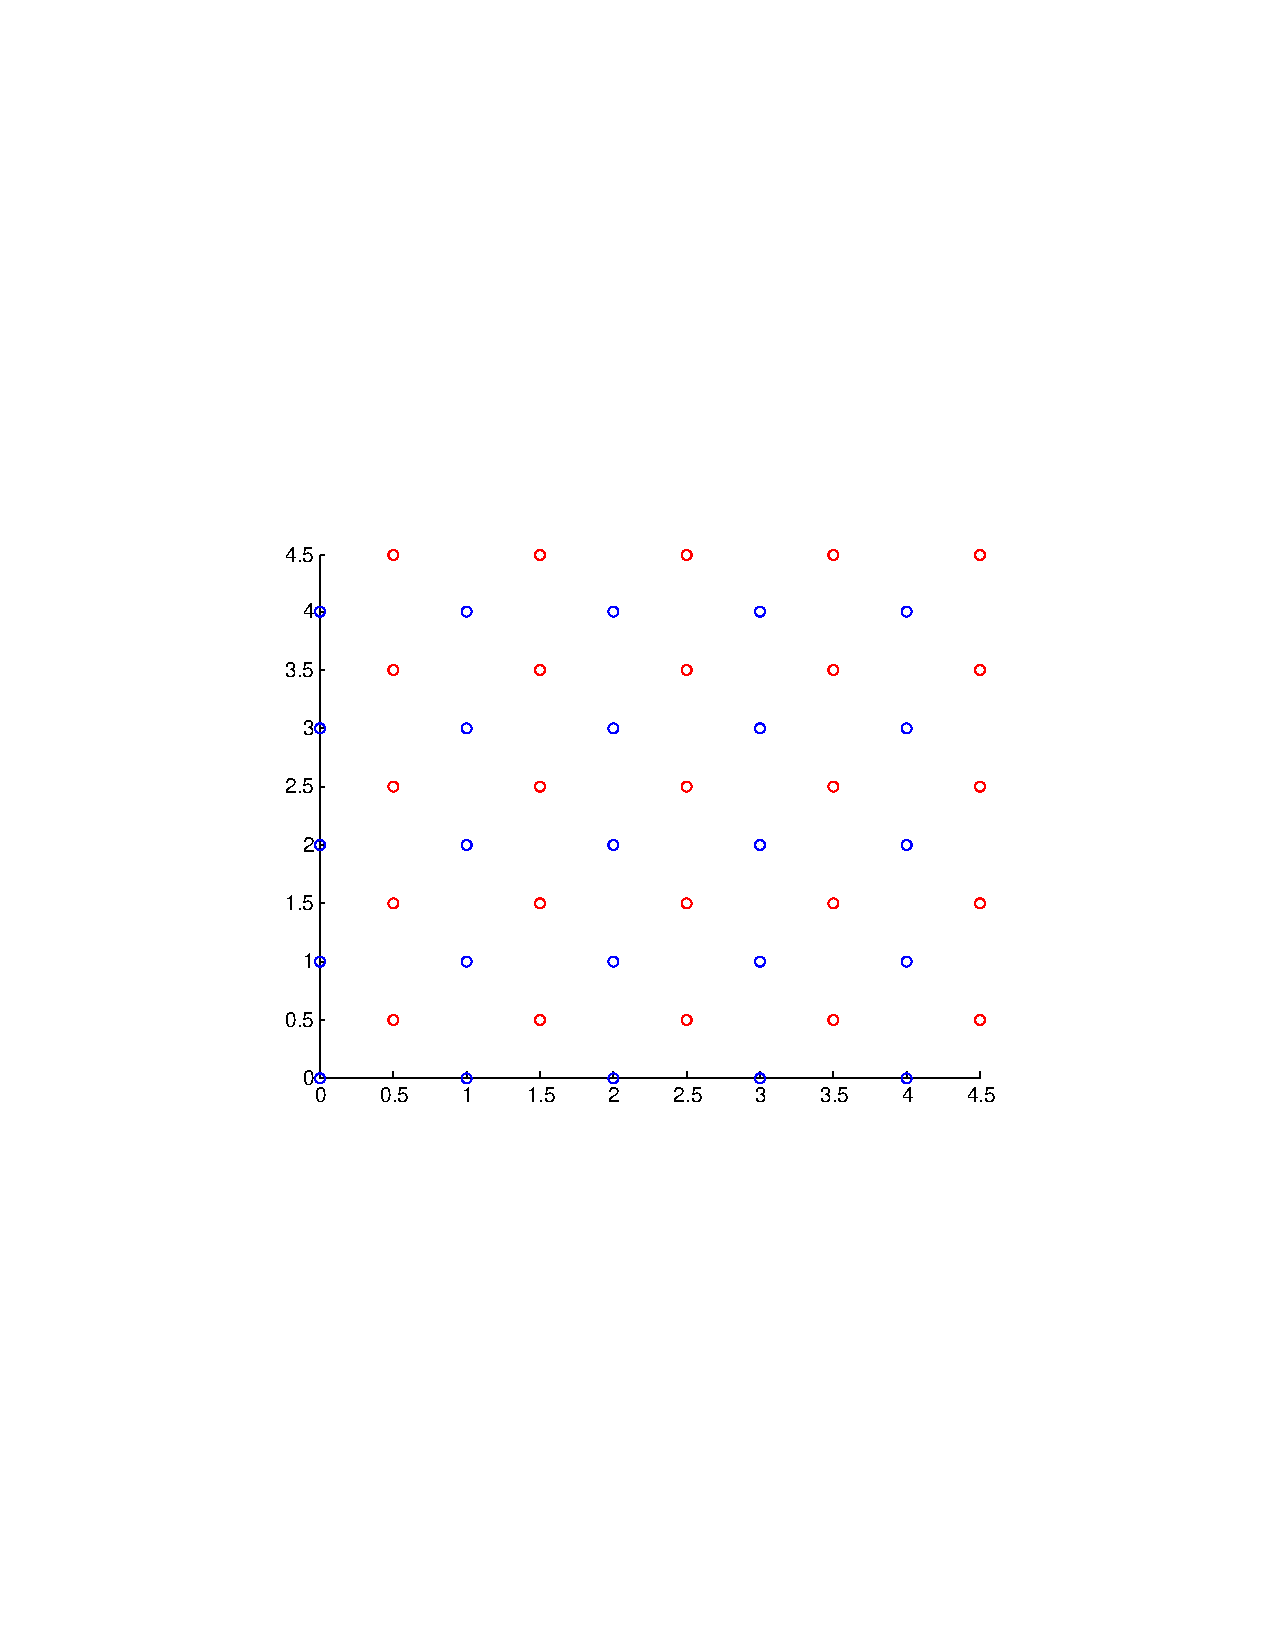
\includegraphics[trim = 20mm 90mm 20mm 90mm,width = 0.5\textwidth,]{Q4plot.pdf}
\end{center}
\end{figure}

\part{b} In the dataset shown in figure \ref{knn}, what is the leave-one-out accuracy of the $k$-NN method when $k=2$? Remember that a data point cannot be considered its own neighbor since it is left out. (Ignore the datapoints that have an output tie for $k=2$ nearest neighbors.)  
\maxmarks{2}
{\color{blue} 2-NN always incorrectly classifies any point other than $(0,0)$, $(4.5, 4.5)$,
since their nearest two neighbors are certain to be labeled differently. The accuracy is {\it zero}. }

\part{c} In this problem, explain briefly why you think $k$-NN performs worse than randomly guessing, which has an accuracy near $50\%$?
\maxmarks{2}

{\color{blue} k-NN's rate of success entirely relies on the data distribution. Usually it is okay 
but we can easily fabricate some distribution to make it extremely inaccurate as shown in this scenario. }

%%%%%%%%%%%%%%%%%%%%%%%%%%%%%%%%%%%%%%%%%%%
\question{6}{A tree about the important things in life. (TA:- \myfirstta)}

The following dataset will be used to learn a decision tree for predicting whether a person is Happy $(H)$ or Sad $(S)$ based on the color of their shoes, whether they wear a wig and the number of ears they have. \\

\begin{table}[h]
	\centering
	\begin{tabular}{|c|c|c|c|}
	\hline
	Color & Wig & Num. Ears & Emotion \\
	\hline
	\hline
	G & Y & 2 & S \\
	G & N & 2 & S \\
	G & Y & 2 & S \\
	B & N & 2 & S \\
	B & N & 2 & H \\
	R & N & 2 & H \\
	R & N & 2 & H \\
	R & N & 2 & H \\
	R & Y & 3 & H \\
	\hline
	\end{tabular}
\end{table}

\part{a} What is Entropy(Emotion $\mid$ Wig=Y)? 
\maxmarks{1} {\color{blue}\[H(E|W=\text{Y})=\sum_E-p(E|W=Y)\log_2p(E|W=Y)=-\frac23\log_2\frac23-\frac13\log_2\frac13=0.92\]}

\part{b} Which attribute would the decision-tree building algorithm choose to use for the root of the tree (assume no pruning)?
\maxmarks{2} {\color{blue} Color. Since 
\[H(E|C)=\frac39\cdot0+\frac29\cdot1+\frac49\cdot0=\frac29\]
\[H(E|W)=\frac39\cdot0.92+\frac69\cdot0.92=0.92\]
\[H(E|N)=\frac89\cdot1+\frac19\cdot0=\frac89\]}

\part{c} Draw the full decision tree that would be learned for this data (assume no pruning).
\maxmarks{3}
\begin{center}
\color{blue}
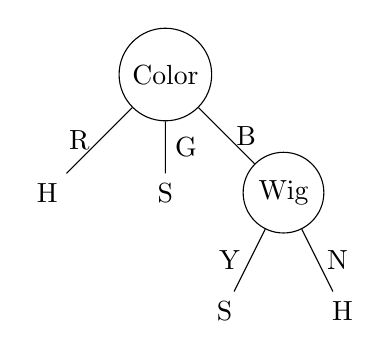
\begin{tikzpicture}
  \node [circle, draw] (color) {Color}
    child {node (h2) {H}
      edge from parent node[left] {R}}
    child {node (s1) {S}
      edge from parent node[right] {G}}
    child {node [circle, draw] (wig) {Wig}
      child {node (s2) {S}
       edge from parent node [left] {Y}}
      child {node (h1) {H}
       edge from parent node [right] {N}}
        edge from parent
         node[right] {B}};
\end{tikzpicture}
\end{center}


\part{d} What would be the training set error for this dataset? Express your answer as the percentage of records that would be misclassified.
\maxmarks{2} 

{\color{blue} The error is 1/9. The record (B,N,2,S) would be misclassified. }

%%%%%%%%%%%%%%%%%%%%%%%%%%%%%%%%%%%%%%%%%%%
\question{7}{Digging up the dense binary tree. (TA:- \myfirstta)}

Consider the following data with three binary attributes, where $x^i$ denotes the $i^{th}$ datapoint, $x_j$ denotes the $j^{th}$ feature of the datapoint, and $y$ denotes the class label:-

\begin{center}
\begin{tabular}{|l|l|l|l|l|}
\hline
& $x_1$ & $x_2$ & $x_3$ & y \\ \hline 	\hline
$x^0$ & 0 & 0 & 0 & 0 \\
$x^1$ & 0 & 0 & 1 & 1 \\
$x^2$ & 0 & 1 & 0 & 1 \\
$x^3$ & 0 & 1 & 1 & 0 \\
$x^4$ & 1 & 0 & 0 & 1 \\
$x^5$ & 1 & 0 & 1 & 0 \\
$x^6$ & 1 & 1 & 0 & 0 \\
$x^7$ & 1 & 1 & 1 & 1 \\
\hline
\end{tabular}
\end{center}

\part{a} Draw the decision tree for the above dataset using the entropy criterion to decide node splits (assume no pruning).
\maxmarks{3}

\begin{center}\color{blue}
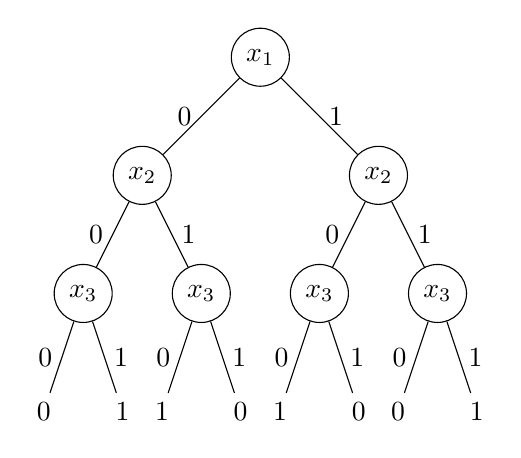
\begin{tikzpicture}
	\tikzstyle{level 1}=[sibling distance=30mm]
	\tikzstyle{level 2}=[sibling distance=15mm]
	\tikzstyle{level 3}=[sibling distance=10mm]
	\node [circle, draw] (x1) {$x_1$}
	  child {node [circle, draw] (x2-1) {$x_2$} 
	    child {node [circle, draw] (x3-1) {$x_3$} 
	      child {node {0} edge from parent node[left] {0} }
	      child {node {1} edge from parent node[right] {1} }
	    edge from parent node[left] {0}}
	    child {node [circle, draw] (x3-2) {$x_3$} 
	      child {node {1} edge from parent node[left] {0} }
	      child {node {0} edge from parent node[right] {1} }
	    edge from parent node[right] {1}}
	  edge from parent node[left] {0}}
     child {node [circle, draw] (x2-1) {$x_2$} 
	    child {node [circle, draw] (x3-1) {$x_3$} 
	      child {node {1} edge from parent node[left] {0} }
	      child {node {0} edge from parent node[right] {1} }
	    edge from parent node[left] {0}}
	    child {node [circle, draw] (x3-2) {$x_3$} 
	      child {node {0} edge from parent node[left] {0} }
	      child {node {1} edge from parent node[right] {1} }
	    edge from parent node[right] {1}}
	  edge from parent node[right] {1}};
\end{tikzpicture}
\end{center}

\part{b} Decision trees are often pruned so that they can better generalize for prediction on the test set. Do you think you could prune any of the lower levels of the above decision tree used to predict the XOR of 3 binary digits? Give reasons for your decision.
\maxmarks{2} {\color{blue} No. We don't know $y$ unless we've tested every single $x_i$.}

\part{c} Considering a generalization of the above problem, let's say that we train a decision tree without any pruning to output the XOR function using \emph{all} possible binary strings of length $n$. Out of the decision tree and KNN classifier (using $l_1$ distance and $k=1$), which one would be more accurate when the test samples are also binary strings of length $n$?
\maxmarks{2} {\color{blue} The decision tree would be 100\% accurate. For k-NN, if a data point can be its own neighbor, then it's 100\% accurate as well;
but if we're talking about leave-one-out accuracy, it will be slightly worse than 100\%. Therefore generally the decision tree is considered to be more accurate. }

\part{d} Out of the decision tree and KNN classifiers considered in the previous question, which one will take lesser time to predict the output label of a new test datapoint? Why? (Hint: Note that there are $2^n$ possible datapoints due to $n$ binary input features. Consider the number of nodes traversed by the decision tree and the number of distance computations performed by the KNN classifier to predict the label of a test datapoint with $n$ binary input features.)
\maxmarks{2} 

{\color{blue} Exactly $n$ nodes are traversed by the decision tree. The k-NN classifier need to iterate through all $2^n$ data points and make $n$ computations for each feature.
So the decision tree will take less time. }

%%%%%%%%%%%%%%%%%%%%%%%%%%%%%%%%%%%%%%%%%%%
\question{8}{On the hardness of learning optimal binary decision trees (TA:- \myfirstta)}

In figure \ref{decision_tree}, assume that the rectangular region consisting of two features $x_1$ and $x_2$ is densely packed with points. The red, green, and yellow subrectangles represent the three classes $C_1, C_2, \text{ and } C_3$ of datapoints. The $x_1 \text{ X } x_2$ dimensions of the red, green, and yellow rectangles are $1\text{ X }6$, $7\text{ X }3$, and $7\text{ X }3$ respectively. The red rectangle is uniformly populated with 6,000 datapoints of class $C_1$. The green rectangle is uniformly populated with 42,000 datapoints of class $C_2$. The yellow rectangle is uniformly populated with 42,000 datapoints of class $C_3$.

\begin{figure}[h!]

\begin{center}
\caption{A 2D dataset with three classes}
\label{decision_tree}
\vspace{4 mm}
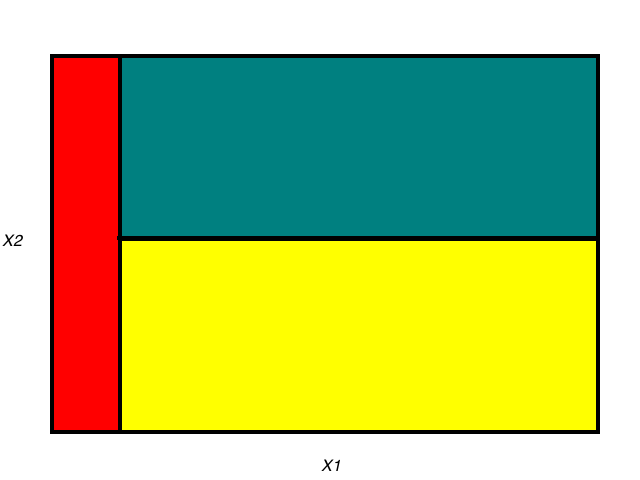
\includegraphics[width=0.5\textwidth]{decision_tree_1}
\end{center}
\end{figure}

\part{a} What is the minimum number of nodes that a decision tree needs to have in order to classify the above dataset correctly?
\maxmarks{2} 

{\color{blue}2. Refer to the tree on the left on the next page.

\begin{center}
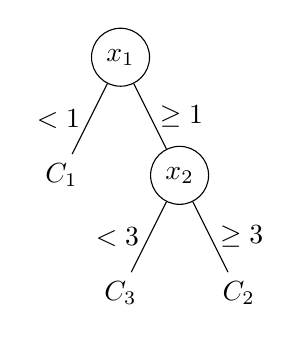
\begin{tikzpicture}
	\node [circle, draw] {$x_1$} 
	  child {node {$C_1$}
	    edge from parent node [left] {$<1$}}
	  child {node [circle, draw] {$x_2$}
	    child {node {$C_3$}
	      edge from parent node [left] {$<3$}}
	    child {node {$C_2$}
	      edge from parent node [right] {$\ge3$}}
	    edge from parent node [right] {$\ge1$}};
\end{tikzpicture}
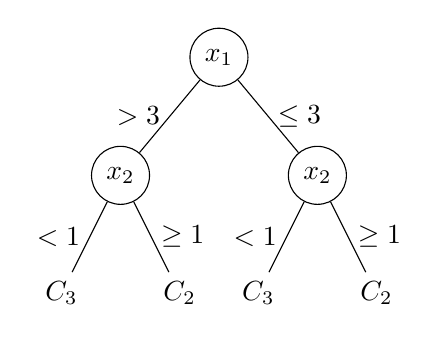
\begin{tikzpicture}
	\tikzstyle{level 1}=[sibling distance=25mm]
	\tikzstyle{level 2}=[sibling distance=15mm]
	\tikzstyle{level 3}=[sibling distance=10mm]
	\node [circle, draw] {$x_1$} 
	  child {node [circle, draw] {$x_2$}
	    child {node {$C_3$}
	      edge from parent node [left] {$<1$}}
	    child {node {$C_2$}
	      edge from parent node [right] {$\ge1$}}
	    edge from parent node [left] {$>3$}}
	  child {node [circle, draw] {$x_2$}
	    child {node {$C_3$}
	      edge from parent node [left] {$<1$}}
	    child {node {$C_2$}
	      edge from parent node [right] {$\ge1$}}
	    edge from parent node [right] {$\le3$}};
\end{tikzpicture}
\end{center}

}


\part{b} What is the number of nodes in the decision tree trained on the above dataset using the entropy criterion?
\maxmarks{2}

{\color{blue}3. Refer to the tree on the right. }

\part{c} Are the number of nodes in the two cases identical or different? Why do you think that is?
\maxmarks{3}

{\color{blue} Different. Entropy criterion only care about optimizing a split at a specific level, and the 
optimal tree considers all splits as a whole.}

\part{d} Construct another toy dataset where the entropy gain criterion leads to a suboptimal decision tree i.e. one with more nodes than another tree of comparable accuracy. Your dataset should have at least four labels and be sufficiently different from the given toy dataset.
\maxmarks{3} 

{\color{blue}
\begin{center}
\begin{tabular}{ccc}
	Color & Glasses & OS \\ \hline
	R & Y & Windows \\
	R & N & Windows \\
	G & Y & Other \\
	G & N & Other \\
	B & Y & Mac OS X \\
	B & Y & Mac OS X \\
	... & ... & Mac OS X \\
	B & N & Ubuntu \\
	B & N & Ubuntu \\
	... & ... & Ubuntu \\
\end{tabular}
\end{center}
Note: the data (B, Y: Mac OS X) appear 48 times, and the data (B, N: Ubuntu) appear 48 times. 
So there are a total of 100 data points.}

\part{e} For your suggested dataset, draw the optimal decision tree as well as the decision tree obtained using the entropy minimization criterion.
\maxmarks{3} 

{\color{blue}
The tree on the left is constructed using entropy criterion, and the right one is optimal.\\
Notations: G = Glasses, C = Color, W = Windows, O = Other, M = Mac OS X, U = Ubuntu.

\begin{center}
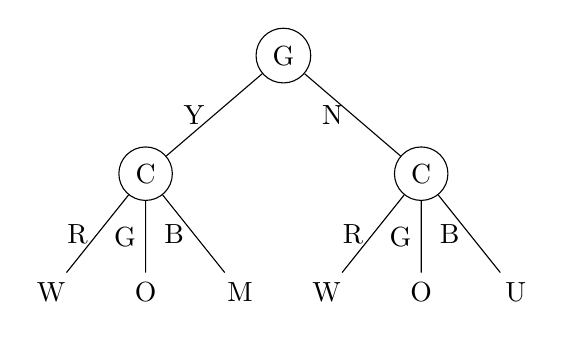
\begin{tikzpicture}
	\tikzstyle{level 1}=[sibling distance=35mm]
	\tikzstyle{level 2}=[sibling distance=12mm]
	\node [circle, draw] {G}
	  child {node [circle, draw] {C}
	    	  child {node {W}
	    	    edge from parent node [left] {R}}
	    	  child {node {O}
	    	    edge from parent node [left] {G}}
	    	  child {node {M}
	    	    edge from parent node [left] {B}}
        edge from parent node [left] {Y}}
	  child {node [circle, draw] {C}
	    	  child {node {W}
	    	    edge from parent node [left] {R}}
	    	  child {node {O}
	    	    edge from parent node [left] {G}}
	    	  child {node {U}
	    	    edge from parent node [left] {B}}
        edge from parent node [left] {N}};
\end{tikzpicture}
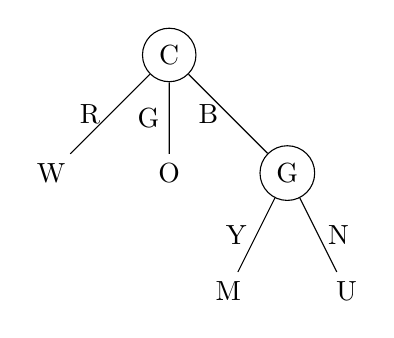
\begin{tikzpicture}
	\tikzstyle{level 1}=[sibling distance=15mm]
	\tikzstyle{level 2}=[sibling distance=15mm]
	\node [circle, draw] {C} 
	    	  child {node {W}
	    	    edge from parent node [left] {R}}
	    	  child {node {O}
	    	    edge from parent node [left] {G}}
	    	  child {node [circle, draw] {G}
	    	     child { node {M} edge from parent node [left] {Y}}
	    	     child { node {U} edge from parent node [right] {N}}
	    	    edge from parent node [left] {B}};
\end{tikzpicture}
\end{center}

}

\part{f} A decision tree can classify the dataset in figure \ref{decision_tree} with 100\% test accuracy (assuming that there is no label noise). What are the general conditions on a dataset under which a decision tree can provide 100\% test accuracy? (Hint: Each internal node of a decision tree performs a split based on a single feature. Think about the class of separation functions such a decision tree entails.)
\maxmarks{3} 

{\color{blue} There are no data that are identically labeled and share exactly the same attribute values. }

\dumptotal

\end{document}

